% Preamble
\documentclass{hnu}

% Packages
\usepackage{graphicx}
\usepackage{overpic}
\usepackage{ulem}
\usepackage{fontspec}
\usepackage{multirow} %表格内跨行
\usepackage{threeparttable}% 三线表
\usepackage{enumitem}
%\setlist[enumerate]{itemsep=0.5\baselineskip}

\newcommand\obs[1]{\textcolor{blue}{#1}} %文本高亮
\newcommand\rev[1]{\textcolor{red}{#1}} %文本高亮
\newcommand\ve[1]{\boldsymbol{#1}} %矢量
\newcommand\bm[1]{\boldsymbol{#1}} % 加粗符号
\newcommand\ma[1]{\mathbf{#1}} % 矩阵，张量等
\newcommand\Dt[2][t]{\frac{\mathrm{D}{#2}}{\mathrm{D}#1}} %物质倒数
\newcommand\dt[2][t]{\frac{\mathrm{d}{#2}}{\mathrm{d}#1}} %微分导数
\newcommand\ppx[2][x]{\frac{\partial {#2}}{\partial {#1}}} %偏导

% Document
\begin{document}
    \createCover % 封面

    \frontmatter
    \createCopyright % 版权

    % ========================================摘要部分
    \begin{abstractCN}
毕业设计（论文）是培养学生综合运用本学科的基本理论、专业知识和基本技能，提高分析和解决实际问题的能力，完成初步培养从事科学研究工作和专业工程技术工作基本训练的重要环节。为了统一和规范我校本科生毕业设计（论文）的写作，保证我校本科生毕业设计（论文）的质量，根据《中华人民共和国国家标准学位论文编写规则》（国家标准GBT7713.1-2006）的规定及学校相关文件要求，特制定《湖南大学机械与运载工程学院本科毕业设计（论文）撰写规范》

    \keywordsCN 湖南大学；机械与运载工程学院；毕业论文
\end{abstractCN}

\begin{abstractENG}
Graduation design (thesis) is a crucial component in fostering students' ability to comprehensively apply the fundamental theories, professional knowledge, and basic skills of their discipline. It aims to enhance their capacity to analyze and solve practical problems and serves as a fundamental training for their future engagement in scientific research and professional engineering and technical work. To standardize and regulate the writing of graduation design (thesis) for undergraduates at our university, and to ensure the quality of their graduation design (thesis), we have specifically formulated the "Writing Guidelines for Undergraduate Graduation Design (Thesis) of the School of Mechanical and Vehicle Engineering, Hunan University" in accordance with the provisions of the "National Standard of the People's Republic of China for the Compilation Rules of Academic Degree Thesis" (National Standard GBT7713.1-2006) and relevant school documents



    \keywordsENG Hunan University; School of Mechanical and Vehicle Engineering; Graduation Thesis
\end{abstractENG}
    % ========================================摘要部分

    \createTOC % 目录
    \createLOF % 插图索引
    \createLOT % 附表索引

    \mainmatter
    % ========================================正文部分
    \chapter{论文构成}
学位论文包括前置部分、正文部分、附录部分、附件。具体构成如图\ref{fig:struct}：
\begin{figure}[htbp]
\centering
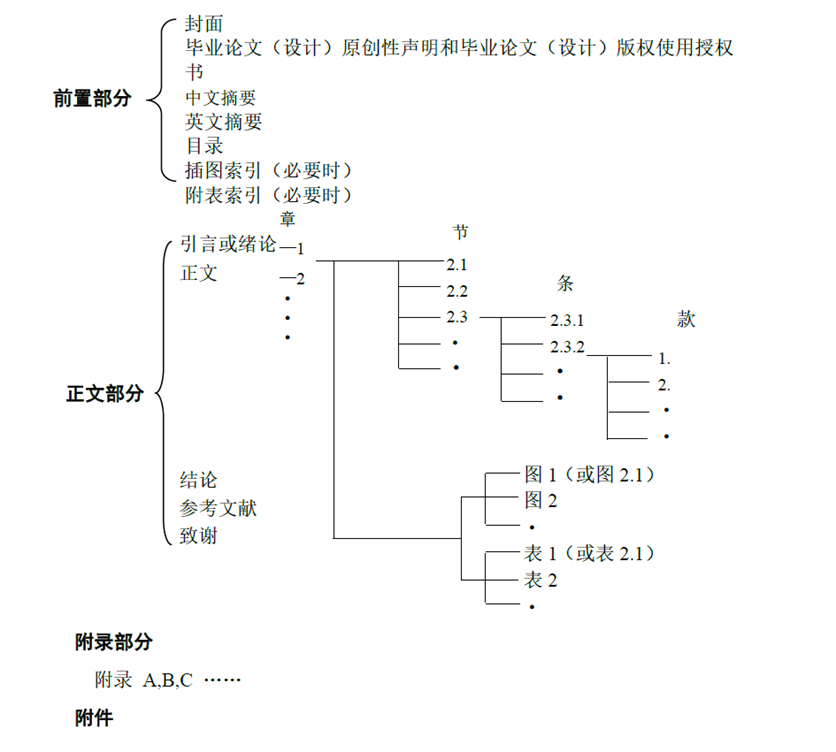
\includegraphics[width=\linewidth]{docs/imgs/structure}
\caption{论文结构与框架}\label{fig:struct}
\end{figure}

    \chapter{内容要求}
\section{论文题目}
题目应该简短、明确、有概括性。通过题目，能大致了解论文内容、专业特点和学科范畴。但字数要适当，一般不宜超过20字。必要时可加副标题。

\section{摘要与关键词}
\subsection{论文摘要}
摘要应概括反映出毕业设计（论文）的内容、方法、成果和结论。摘要中一般不宜使用公式、图表，不标注引用文献编号。中文摘要以300左右字为宜、外文摘要以250个实词左右为宜。

\subsection{关键词}
关键词是供检索用的主题词条，应采用能覆盖设计（论文）主要内容的通用技术词条（参照相应的技术术语标准），尽量从《汉语主题词表》中选用，未被词表收录的新学科、新技术中的重要术语和地区、人物、文献等名称，也可作为关键词标注。关键词一般为3～5个，按词条的外延层次排列（外延大的排在前面）。关键词应以与正文不同的字体字号编排在摘要下方。多个关键词之间用分号分隔。中英文关键词应一一对应。

\section{目录}
目录按章、节、条三级标题编写，要求标题层次清晰。目录中的标题要与正文中标题一致。目录中应包括绪论、报告（论文）主体、结论、致谢、参考文献、附录等。

\section{正文}
正文是毕业设计(论文)的主体和核心部分，一般应包括绪论、报告（论文）主体及结论等部分。

\subsection{绪论}
绪论一般作为第一章，是毕业论文(设计)主体的开端。绪论应包括：毕业论文（设计）的背景及目的；国内外研究状况和相关领域中已有的成果；设计和研究方法；设计过程及研究内容等。绪论一般不少于1.5千字。

\subsection{主体}
主体是毕业论文(设计)的主要部分，应该结构合理、层次清楚、重点突出、文字简练、通顺。主体的内容应包括以下各方面：
\begin{enumerate}
	\item 毕业论文(设计)总体方案设计与选择的论证。	
	\item 毕业论文(设计)各部分（包括硬件与软件）的设计计算。
	\item 试验方案设计的可行性、有效性以及试验数据的处理及分析。
	\item 对本研究内容及成果进行较全面、客观的理论阐述，应着重指出本研究内容中的创新、改进与实际应用之处。理论分析中，应将他人研究成果单独书写，并注明出处，不得将其与本人的理论分析混淆在一起。对于将其他领域的理论、结果引用到本研究领域者，应说明该理论的出处，并论述引用的可行性与有效性。
	\item 自然科学的论文应推理正确，结论清晰，无科学性错误。
	\item 管理和人文学科的论文应包括对所研究问题的论述及系统分析、比较研究，模型或方案设计，案例论证或实证分析，模型运行的结果分析或建议、改进措施等。
\end{enumerate}

\subsection{结论}
结论是毕业论文(设计)的总结，是整篇设计报告（论文）的归宿。要求精炼、准确地阐述自己的创造性工作或新的见解及其意义和作用，还可进一步提出需要讨论的问题和建议。

\section{参考文献}
按正文中出现的顺序列出直接引用的主要参考文献。

毕业论文(设计)的撰写应本着严谨求实的科学态度，凡有引用他人成果之处，均应按论文中所出现的先后次序列于参考文献中。并且只列出正文中以标注形式引用或参考的有关著作和论文。一篇论著在论文中多处引用时，在参考文献中只能出现一次，序号以第一次出现的位置为准。

\section{致谢}
致谢中主要感谢导师和对论文工作有直接贡献及帮助的人士和单位。

\section{附录}
对于一些不宜放入正文中、但作为毕业论文(设计)又是不可缺少的部分，或有重要参考价值的内容，可编入毕业论文(设计)的附录中。例如，过长的公式推导、重复性的数据、图表、程序全文及其说明等。
    \chapter{书写规范与打印要求}
\section{文字和字数}
一般用汉语简化文字书写，字数在1.2万字左右，报告（内容）或软件说明书，字数在1万字左右。

\section{书写}
论文一律由本人在计算机上输入、编排并打印在A4幅面白纸上。毕业论文（设计）前置部分（即正文之前）一律用单面印刷，正文部分开始双面印刷。致谢和附录部分应单面起页双面印刷（如正文结束页为单页，则单数页背面不加页眉和页码，致谢单面起页，如致谢为单页，其背面亦不加页眉和页码）。

\section{字体和字号}
论~~文~~题目：\hspace{2cm}小2号黑体

章~~~~标~~~~题：\hspace{2cm}3号黑体

节~~~~标~~~~题：\hspace{2cm}小4号黑体

条~~~~标~~~~题：\hspace{2cm}小4号黑体

正~~~~~~~~~~~~文：\hspace{2cm}小4号宋体

页~~~~~~~~~~~~码：\hspace{2cm}5号宋体

数字和字母：\hspace{2cm}Times New Roman体

\section{封面}
毕业论文（设计）封面规范（见样张1），论文封皮一律采用白色铜版纸，封皮大小为A4规格。

\section{原创性声明及授权书}
见样张2。

\section{论文页面设置}
\subsection{页眉}
页眉为\uline{~~~~~~~~湖南大学本科生毕业论文（设计）~~~~~~~~}。

\subsection{页边距}
上边距：30mm；下边距：25mm；左边距：30mm；右边距：20mm；行间距为1.5倍行距。

\subsection{页码的书写要求}
论文页码从绪论部分开始，至附录，用阿拉伯数字连续编排，页码位于页脚居中。封面、摘要和目录不编入论文页码；摘要和目录用罗马数字单独编页码。

\section{摘要}
\subsection{中文摘要}
中文摘要包括：论文题目（小3号黑体）、“摘要”字样（3号黑体）、摘要正文(小4号宋体)和关键词。

摘要正文后下空一行打印“关键词”三字（4号黑体），关键词一般为3～5个，每一关键词之间用分号分开，最后一个关键词后不打标点符号。

\subsection{英文摘要}
英文摘要另起一页，其内容及关键词应与中文摘要一致，并要符合英语语法，语句通顺，文字流畅。

英文题目的字样为：The title（小3号 Times New Roman 加粗）

英文摘要字样为：Abstract(3号 Times New Roman 加粗)

然后隔行书写摘要的文字部分。（字体为小4号Times New Roman）

摘要正文后下空一行打印关键词（4号Times New Roman加粗）：key word1；key word2；（关键词3－5个，小4号Times New Roman加粗）

英文和汉语拼音一律为Times New Roman体，字号与中文摘要相同。

\section{目录}
专业目录的三级标题，建议按（1……、1.1……、1.1.1……）的格式编写，目录中各章题序的阿拉伯数字用Times New Roman体，第一级标题用小4号黑体，其余用小4号宋体。目录的打印范例。

\section{论文正文}
\subsection{章节及各章标题}
论文正文分章节撰写，每章应另起一页。各章标题要突出重点、简明扼要。字数一般在15字以内，不得使用标点符号。标题中尽量不采用英文缩写词，对必须采用者，应使用本行业的通用缩写词。

\subsection{层次}
层次以少为宜，根据实际需要选择。正文层次的编排和代号要求统一，层次为章（如“1”）（3号黑体）、节（如“1.1”）、条（如“1.1.1”）、款（如“（1）”）。层次用到哪一层次视需要而定，若节后无需“条”时可直接列“款”、“项”。“节”、“条”的段前、段后各设为0.5行。

\section{引用文献}
引用文献标示方式应全文统一，并采用所在学科领域内通用的方式，所引文献编号用阿拉伯数字置于方括号中，用上标的形式置于所引内容最末句的右上角，如：“…成果$^{[1]}$”，引用文献应与文中标注一致。几处地方引用同一个文献时，文中标注按第一次出现的序号。当提及的参考文献为文中直接说明时，其序号应该用阿拉伯数字与正文排齐，如“由文献[8, 10-14]可知”。

不得将引用文献标示置于各级标题处。

\section{名词术语}
科技名词术语及设备、元件的名称，应采用国家标准或部颁标准中规定的术语或名称。标准中未规定的术语要采用行业通用术语或名称。全文名词术语必须统一。一些特殊名词或新名词应在适当位置加以说明或注解。

采用英语缩写词时，除本行业广泛应用的通用缩写词外，文中第一次出现的缩写词应该用括号注明英文全文。

\section{物理量名称、符号与计量单位}
\subsection{物理量的名称和符号}
物理量的名称和符号应符合GB3100~3102-86的规定。论文中某一量的名称和符号应统一。

\subsection{物理量计量单位}
物理量计量单位及符号应按国务院1984年发布的《中华人民共和国法定计量单位》及GB3100\~3102执行，不得使用非法定计量单位及符号。计量单位符号，除用人名命名的单位第一个字母用大写之外，其它一律用小写字母。

非物理量单位（如件、台、人、元、次等）可以采用汉字与单位符号混写的方式，如“万t·km”。

文稿叙述中不定数字之后允许用中文计量单位符号，如“几千克至1000kg”。

表达时刻时应采用中文计量单位，如“上午8点3刻”，不能写成“8h45min”。

计量单位符号一律用正体。

\section{外文字母的正、斜体用法}
物理量符号、物理常量、变量符号用斜体，计量单位等符号均用正体。

\section{数字}
除习惯用中文数字表示的以外，一般均采用阿拉伯数字。年份一概写全数，如2003年不能写成03年。

\section{公式}
公式应另起一行写在稿纸中央，公式和编号之间不加虚线。公式较长时最好在等号“＝”处转行，如难实现，则可在＋、－、×、÷运算符号处转行，运算符号应写在转行后的行首，公式的编号用圆括号括起来放在公式右边行末。

公式序号按章编排，如第一章第一个公式序号为“(1.1)”，附录A中的第一个公式为“(A1)”等。

文中引用公式时，一般用“见式(1.1)”或“由公式(1.1)”。

公式中用斜线表示“除”的关系时应采用括号，以免含糊不清，如a/(bcosx)。通常“乘”的关系在前，如acosx/b而不写成(a/b)cosx。

\section{表格}
每个表格应有的表序和表题。并应在文中进行说明，例如：“如表1.1”。

表序一般按章编排，如第一章第一个插表的序号为“表1.1”等。表序与表名之间空一格，表名中不允许使用标点符号，表名后不加标点。表序与表名置于表上居中（5号黑体加粗，数字和字母为5号Times New Roman体加粗）。

表头设计应简单明了，尽量不用斜线。表头与表格为一整体，不得拆开排写于两页。

全表如用同一单位，将单位符号移至表头右上角。

表中数据应正确无误，书写清楚。数字空缺的格内加“－”字线（占2个数字），不允许用“²”、“同上”之类的写法。

表内文字说明（5号宋体），起行空一格、转行顶格、句末不加标点。

表中若有附注时，用小5号宋体，写在表的下方，句末加标点。仅有一条附注时写成：注：；

有多条附注时，附注各项的序号一律用阿拉伯数字，例如：注1。

\section{图}
毕业设计的插图应与文字紧密配合，文图相符，技术内容正确。选图要力求精练。

\subsection{制图标准}
插图应符合国家标准及专业标准。

机械工程图：采用第一角投影法，严格按照GB4457~4460-84，GB131-83《机械制图》标准规定。

电气图：图形符号、文字符号等应符合有关标准的规定。

流程图：原则上应采用结构化程序并正确运用流程框图。

对无规定符号的图形应采用该行业的常用画法。

\subsection{图题及图中说明}
每幅插图均应有图题（由图号和图名组成）。图号按章编排，如第一章第一图的图号为“图1.1”等。图题置于图下，用5号宋体加粗。有图注或其他说明时应置于图题之上，用小5号宋体。图名在图号之后空一格排写。引用图应说明出处，在图题右上角加引用文献号。图中若有分图时，分图号用(a)、(b)等置于分图之下。

图中各部分说明应采用中文（引用的外文图除外）或数字符号，各项文字说明置于图题之上（有分图题者，置于分图题之上）。
\subsection{插图编排}
插图与其图题为一个整体，不得拆开排写于两页。插图处的该页空白不够排写该图整体时，可将其后文字部分提前排写，将图移至次页最前面。
\subsection{坐标与坐标单位}
对坐标轴必须进行说明，有数字标注的坐标图，必须注明坐标单位。
\subsection{论文原件中照片图及插图}
毕业设计(论文)原件中的照片图应是直接用数码相机拍照的照片，或是原版照片粘贴，不得采用复印方式。照片可为黑白或彩色，应主题突出、层次分明、清晰整洁、反差适中。照片采用光面相纸，不宜用布纹相纸。对金相显微组织照片必须注明放大倍数。

\section{注释}
毕业设计（论文）中有个别名词或情况需要解释时，可加注说明，注释可用页末注（将注文放在加注页稿纸的下端）或篇末注（将全部注文集中在文章末尾），而不用行中注（夹在正文中的注）。若在同一页中有两个以上的注时，按各注出现的先后编列注号，注释只限于写在注释符号出现的同页，不得隔页。

\section{参考文献}
参考文献的著录均应符合国家有关标准（按GB7714—2015《信息与文献参考文献著录规则》执行）。详见附件《参考文献示例》。

关于参考文献的未尽事项可参见国家标准《信息与文献参考文献著录规则》（GB7714－2015）。

\section{……}
其他部分请自行阅读学院颁布的撰写规范文件。
    % ========================================正文部分

    % 参考文献
    \createBibliography
    \bibliography{refs}  % 参考文献使用 BibTeX 编译

    % ========================================致谢部分
    \begin{newThanks}
    致谢中主要感谢导师和对论文工作有直接贡献及帮助的人士和单位\ldots
\end{newThanks}
    % ========================================致谢部分

    % 附录
    \createAppendix
    % ========================================附录部分
    \input{docs/appendices/appendix1}
    \section{图表示例}
由于该模板服务于湖南大学机械与运载工程学院于2025年末发布的新的本科生毕业论文撰写规范（适用于2026年毕业生），为了实现撰写规范中的一些要求，新定义了一些命令。在此处将这些命令和一些其他常用的命令进行一些演示和说明。

首先是表注：
\begin{table}[ht]
    \abovetopsep=0pt
    \aboverulesep=0pt
    \belowrulesep=0pt
    \belowbottomsep=0pt
    \begingroup
    \centering
    \caption{获奖}
    \label{tab:table1}
    \fontSimsun\sizeFive
    \newcolumntype{Z}{>{\centering\arraybackslash}X}
    \begin{tabularx}{\textwidth}{Z|Z|Z|Z}
        \toprule
        年份                    & 奖项                                              & 类别         & 结果 \\
        \hline
        2022                  & 金摇杆奖                                            & 最受期待游戏     & 提名 \\
        \hline
        \multirow{6}{*}{2023} & 2023世界科幻游戏年度大奖                                  & 最佳人气奖      & 获奖 \\
        \cline{2-4}
        & \multirow{3}{0.25\textwidth}{Google Play年度最佳榜单} & 最佳游戏       & 获奖 \\
        \cline{3-4}
        &                                                 & 最佳剧情游戏     & 获奖 \\
        \cline{3-4}
        &                                                 & 最佳平板游戏     & 获奖 \\
        \cline{2-4}
        & App Store Awards                                & 年度iPhone游戏 & 获奖 \\
        \cline{2-4}
        & 2023年游戏大奖                                       & 最佳手机游戏     & 获奖 \\
        \bottomrule
    \end{tabularx}
    \endgroup

    \vspace{3pt}
    \fontSimsun\sizeFivel 注：仅供参考。
    \vspace{-15pt}
\end{table}

本来定义了表注的命令tablenotes，但是有一些bug，修复半天修复不了，懒得搞了，所以直接定义字体和大小吧。

然后是三线表：
\begin{table}[htbp]
    \abovetopsep=0pt
    \aboverulesep=0pt
    \belowrulesep=0pt
    \belowbottomsep=0pt
	\centering
	\begin{threeparttable}[c]
		\caption{三线表}
		\label{tab:ch1-part-rotate}
		\tableBodyFont
        \begin{tabular}{lcc}
			\toprule
			换热器  & 热边压降损失    & 冷边压降损失               \\
			\midrule
			初级&2974.37&2931.52\\
			次级&2924.65&3789.76\\
			\bottomrule  
		\end{tabular}
	\end{threeparttable}
\end{table}

其次是行内文献引用：

“设定L3下表面固定，上表面施加0.2 MPa的均匀压力载荷，计算其轴向压缩响应。计算得出单椎体轴向等效刚度约为8200 N/mm，符合健康年轻男性裸椎的高刚度特征。通过与文献\inlinecite{nekkanty2010stiffness}中对尸体进行的实验数据的比对，验证了本文逆向建模边界的准确性与材料参数设置的合理性。此步骤确立了基准模型，可进一步开展后续的双节段系统仿真。”

接下来是分图排版：
\begin{figure}[H]
    \centering
    \begin{subfigure}[b]{0.3\textwidth}
        \centering
        \includegraphics[width=\textwidth]{example-image-a}
        \caption{分图A} 
    \end{subfigure}
    \hfill
    \begin{subfigure}[b]{0.3\textwidth}
        \centering
        \includegraphics[width=\textwidth]{example-image-b}
        \caption{分图B} 
    \end{subfigure}
    \caption{总图名}
\end{figure}

第二类分图排版：
\begin{figure}[H]
    \centering
    \subfloat[这是啥]{\label{1} 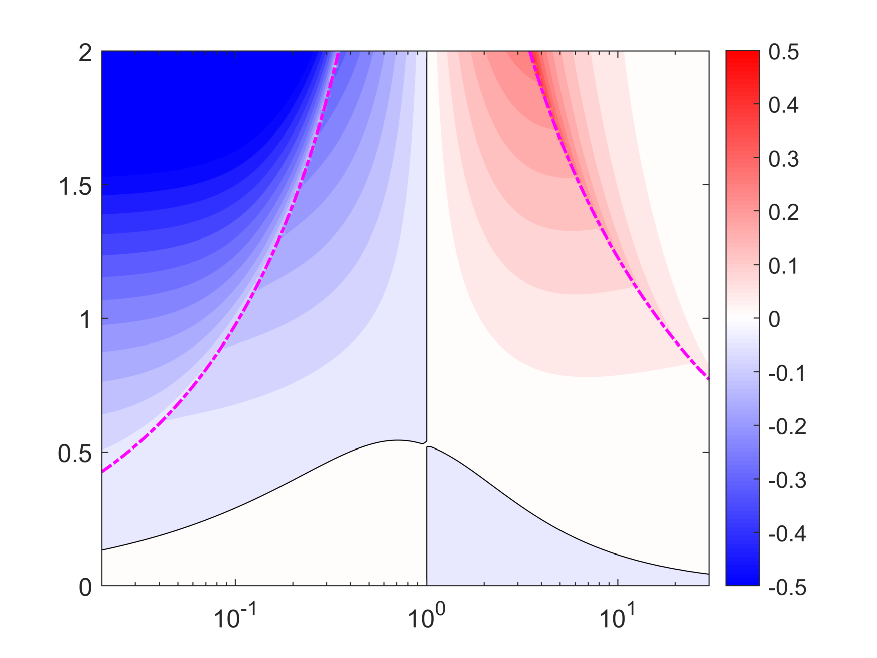
\includegraphics[width=0.5\linewidth]{docs/imgs/overpic_example}}
    \subfloat[这又是啥]{\label{2} 
\includegraphics[width=0.35\linewidth]{docs/imgs/HSR}}
    \caption{分图2}
    \label{不知道是啥}
\end{figure}

图注：
\begin{figure}[H]
    \centering
    
\includegraphics[width=100pt]{docs/imgs/herta}
    \figurenotes{这是图注或其他说明。} 
    \caption{签名}
    \label{fig:figure2}
\end{figure}

最后是有序列表：
\begin{enumerate}
    \item \textbf{有序列表1}：有序列表1有序列表1有序列表1有序列表1有序列表1有序列表1有序列表1有序列表1有序列表1有序列表1有序列表1有序列表1有序列表1有序列表1有序列表1有序列表1
    \item \textbf{有序列表2}：有序列表2有序列表2有序列表2有序列表2有序列表2有序列表2有序列表2有序列表2有序列表2有序列表2有序列表2
    \item \textbf{有序列表3}：有序列表3有序列表3有序列表3有序列表3
\end{enumerate}

和无序列表：
\begin{itemize}
    \item \textbf{无序列表1}：无序列表1无序列表1无序列表1无序列表1无序列表1无序列表1无序列表1
    \item \textbf{无序列表2}：无序列表2无序列表2无序列表2无序列表2无序列表2无序列表2无序列表2无序列表2
    \item \textbf{无序列表3}：无序列表3无序列表3无序列表3无序列表3无序列表3
\end{itemize}

其他请自行学习\LaTeX{}。因为\LaTeX{}是世界上最好的语言（误）！推荐阅读：董晟渤\footnote{北京大学，数学科学学院，概率论与数理统计在读博士}的博客内容：《LaTeX：从入门到日常使用》https://dylandong.top/posts/e480。

    \section{代码}

\begin{lstlisting}
print("Hello World!")
\end{lstlisting}
    % ========================================附录部分
\end{document}